\subsubsection{KNN Classifier}

During our initial experimentation, we found that KNN took over 22 hours to predict on our test data set after training - Figure \ref{fig:knn_train}. Additionally, we utilised our second VM machine, and KNN took over 28 hours to predict our test set of data, and subsequently crashed the system multiple times before we could gather results or evidence. KNN's algorithm means it does not build and store a model during training but rather stores them in memory. As a result, when we predict on the test set we encounter a high computational complexity task as KNN searches for the K-nearest neighbour from our training set. As we have a relatively large amount of features, this further increases the computational power required for these tasks. This was deemed too long for real-world applications where detecting network attacks would be time-sensitive. As network attacks can occur quickly, an IDS using ML algorithms need to have a quick response to detecting these attacks.

Whilst KNN has advantages, such as being easy to implement and interpret, given the limitations in hardware, we ultimately prioritised speed and accuracy for this work and decided not to continue with using this classifier and therefore our results for this classifier remain inconclusive.

\medskip

\begin{figure}[h]
\caption{Training Time for KNN Classifier}
\label{fig:knn_train}
\centering
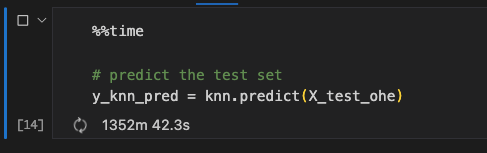
\includegraphics[width=\textwidth]{Appendices/Images/knn_predict-2023-04-15.png}
\end{figure}